\documentclass[handout,xcolor=svgnames]{beamer}
\usepackage[utf8]    {inputenc}
\usepackage[T1]      {fontenc}
\usepackage[english] {babel}
\usepackage{tikz}
\usetikzlibrary{arrows,shapes}
\usepackage{environ}
\usepackage{amsmath,amsfonts,graphicx}
\usepackage{beamerleanprogress}
\newcommand{\hicolor}{darkorange}
\newcommand{\imp}[1]{\begin{center}\Large{\color{\hicolor}{#1}}\end{center}}
\newcommand{\pointout}[1]{{\underline{\textbf{#1}}}}

\tikzset{>=latex}

\title
  [SEE\hspace{2em}]
  {Secure Execution Environment}

\author[]
  {Yogesh Swami}

\date
  {\today}

\institute
  {Cryptography Research,\\a division of Rambus}


\begin{document}

\section{CMv2}

\maketitle

\begin{frame}
  {CMv2 Goals}

  \begin{enumerate}
  \item Flexible security model\pause
  \item Multi-Tenancy\pause
  \item Core Agnostic\pause
  \item Cloud Based Tenant and Agent Management
  \end{enumerate}
\end{frame}


\begin{frame}
  {Flexible Security Model}
 % \imp{Customer should decide the level of security}
  \begin{columns}
    \begin{column}{0.7\textwidth}
    \begin{itemize}
      \item Full Computation Security
      \begin{itemize}
          \item Host assumed to be malicious
          \item Computation, Keys, and Data protected by secure element
      \end{itemize}
      \item Hybrid Data Security
      \begin{itemize}
          \item Computational integrity not a concern
          \item Keys protected by secure element (HSM/Smart Card)
      \end{itemize}
      \item Host Computation Security
      \begin{itemize}
          \item Host runs SEE without any secure element
          \item Host still hardened by CRI!
      \end{itemize}
      \item \pointout{Wish}: Allow seamless transition
    \end{itemize}
    \end{column}

    %% Picture column
    \begin{column}{0.3\textwidth}
    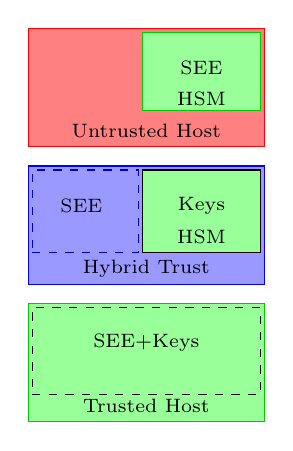
\begin{tikzpicture}
    \draw[fill=red!50,draw=red] (0,3.5) -- (3,3.5) -- (3, 5) -- (0, 5) --cycle;
    \node at (1.5,3.7) {\scriptsize{Untrusted Host}};
    \draw[fill=green!40, draw=green!80!black] (1.45,3.95) -- (2.95,3.95) -- (2.95,4.95) -- (1.45,4.95) -- cycle;
    \node at (2.2,4.1) {\scriptsize{HSM}};
    \node at (2.2,4.5) {\scriptsize{SEE}};

    \draw[fill=blue!40,draw=blue] (0,1.75) -- (3,1.75) -- (3,3.25) -- (0,3.25) -- cycle;
    \node at (1.5,1.95) {\scriptsize{Hybrid Trust}};
    \draw[dashed, fill=blue!40, draw=blue!80!black] (0.05,2.15) -- (1.40,2.15) -- (1.40,3.20) -- (0.05,3.20) -- cycle;
    \draw[fill=green!40, draw=black] (1.45,2.15) -- (2.95,2.15) -- (2.95,3.20) -- (1.45,3.20) -- cycle;
    \node at (0.675,2.75) {\scriptsize{SEE}};
    \node at (2.2,2.75) {\scriptsize{Keys}};
    \node at (2.2,2.35) {\scriptsize{HSM}};

    \draw[fill=green!40,draw=green!80!black] (0,0) -- (3,0) -- (3, 1.5) -- (0, 1.5) --cycle;
    \draw[dashed, fill=green!40, draw=black] (0.05,0.35) -- (2.95,0.35) -- (2.95,1.45) -- (0.05,1.45) -- cycle;
    \node at (1.5,0.2) {\scriptsize{Trusted Host}};
    \node at (1.5,1) {\scriptsize{SEE+Keys}};

    \end{tikzpicture}
    \end{column}
    \end{columns}
\end{frame}


\begin{frame}
  {Multi-Tenancy}
  \imp{Multiple Tenants share the same secure hardware element}
    \begin{itemize}
      \item Secure bootstrapping of tenant's credentials
      \item Secrets remain private to tenant (not even known to SA)
      \item Compute, Memory, Storage and Credentials isolation
    \end{itemize}
\end{frame}


\begin{frame}
  {Core Agnostic}
  \imp{Single infrastructure should support heterogeneous set of cores}
    \begin{itemize}
      \item Facilitate key-management for arbitrary core
      \begin{itemize}
          \item Instruction set known to CRI
          \item Instruction set \underline{not known} to CRI
      \end{itemize}
      \item Provision cores at arbitrary key life cycle
      \begin{itemize}
          \item Cores serialized via CM infra
          \item Cores \underline{not serialized} via CM infra
      \end{itemize}
      \item Support multiple key-exchange, auth/enc, and policies
      \begin{itemize}
          \item Ferguson-Schneier
          \item TLS
          \item IPSec/IKEv(1/2)
          \item (H)MQV
      \end{itemize}
  \end{itemize}
\end{frame}


\begin{frame}
  {Cloud Based}
  \imp{SEE should run across heterogeneous set of hardware platform/secure element}
  \begin{itemize}
      \item Modules/Agents should work seamlessly across different hardware
      \begin{itemize}
          \item HSM (Utimaco/Thales/SafeNet...)
          \item SGX
          \item No secure element
      \end{itemize}
      \item Demand driven load distribution
      \begin{itemize}
          \item Bring up new SEEs as needed
          \item Seamlessly share PCDs/Tickets across SEEs
      \end{itemize}
      \item \pointout{Wish}: Migrate from one hardware platform to another
  \end{itemize}
\end{frame}


\begin{frame}
  {SEE (1)}
  \begin{columns}
  \begin{column}{0.5\textwidth}
  \begin{itemize}
      \item Lightweight Virtual Machine
      \begin{itemize}
          \item SEE interface to Secure Element
          \item Compute Isolation
          \item Memory Isolation
      \end{itemize}
      \item Per-tenant namespace
      \begin{itemize}
          \item Key-db + data isolation
      \end{itemize}
      \item Oracle access to long-term keys
      \begin{itemize}
          \item Use key-handle instead of raw keys
          \item Avoid accidental/malicious key-abuse
          \item Facilitate policy enforcement/accounting
      \end{itemize}
        \end{itemize}
    \end{column}
    \begin{column}{0.5\textwidth}
        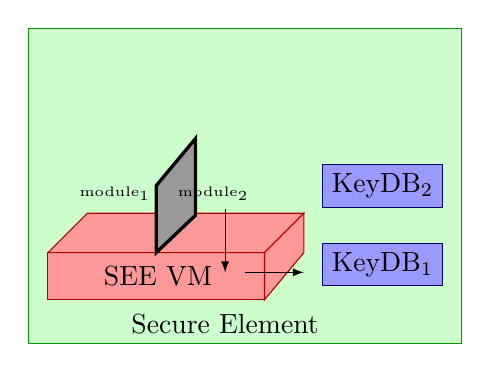
\begin{tikzpicture}
        \draw[fill=green!20,draw=green!60!black] (0,0) -- (5.5,0) -- (5.5, 4) -- (0, 4) --cycle;
        \node at (2.5,0.25) {Secure Element};
        \draw[fill=red!40,draw=red!70!black] (0.25,.55) -- (3,.55) -- (3, 1.15) -- (0.25, 1.15) --cycle;
        \draw[fill=red!40,draw=red!70!black] (0.25,1.15) -- (0.75,1.65) -- (3.5,1.65) -- (3, 1.15) -- cycle;
        \draw[fill=red!40,draw=red!70!black] (3,0.55) -- (3.5,1.15) -- (3.5, 1.65) -- (3, 1.15) -- cycle;
        \draw[very thick, fill=black!40] (1.625,1.15) -- (1.625, 2) -- (2.125,2.6) -- (2.125,1.625) -- cycle;
        \node at (1.65,.85) {SEE VM};
        \node at (1.1,1.9) {\tiny{module$_1$}};
        \node at (2.35,1.9) {\tiny{module$_2$}};
        \node[fill=blue!40,draw=blue!40!black] (keydb) at (4.5, 1) {KeyDB$_1$};
        \node[fill=blue!40,draw=blue!40!black] (keydb) at (4.5, 2) {KeyDB$_2$};
        \draw[draw=black, ->] (2.5,1.7) -- (2.5,0.9);
        \draw[draw=black, ->] (2.75,0.9) -- (3.5,0.9);
        \end{tikzpicture}
    \end{column}
    \end{columns}
\end{frame}

\begin{frame}
  {SEE (2)}
  \begin{columns}
  \begin{column}{0.55\textwidth}
  \begin{itemize}
      \item Support asynchronous, on-demand $Host \leftrightarrow SEE$ interactions
      \begin{itemize}
          \item Multiple round trip $Core \leftrightarrow SEE$ interactions
          \item On demand data load into SEE (give me PCD $0x27364$)
      \end{itemize}
      \item Capabilities based execution
      \begin{itemize}
          \item Explicitly signed token grants access to SEE resources
          \item Deep audit trail
      \end{itemize}
  \end{itemize}
  \end{column}
  \begin{column}{0.45\textwidth}
    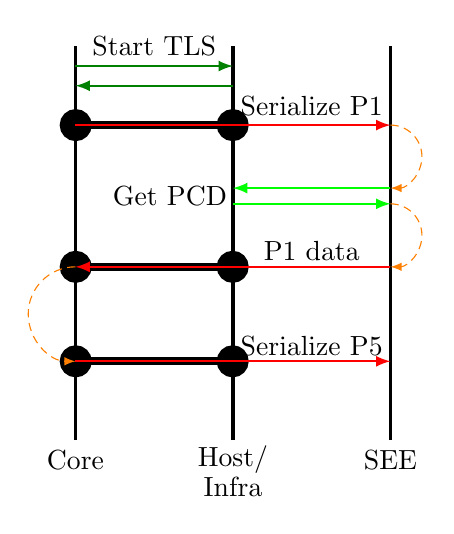
\begin{tikzpicture}
        \draw[draw=black, very thick] (0,0) -- (0,5);
        \node at (0,-0.25) {Core};
        \draw[draw=black, very thick] (2,0) -- (2,5);
        \node at (2,-0.25) {Host/};
        \node at (2,-0.6) {Infra};
        \draw[draw=black, very thick] (4,0) -- (4,5);
        \node at (4,-0.25) {SEE};
        \node at (1,5) {Start TLS};
        \draw[->, thick, draw=green!50!black] (0,4.75) -- (2,4.75);

        \node at (3,4.25) {Serialize P1};
        \draw[<-, thick, draw=green!50!black] (0,4.5) -- (2,4.5);
        \draw[*-*, thick, line width=1mm, draw=black] (-.2,4) -- (2.2,4);
        \draw[->, thick, draw=red] (0,4) -- (4,4);
        \draw[->,densely dashed, orange] (4,4) arc (90:-90:.4);
        \draw[<-, thick, draw=green] (2,3.2) -- (4,3.2);
        \draw[->, thick, draw=green] (2,3) -- (4,3);
        \node at (1.2,3.1) {Get PCD};
        \draw[->,densely dashed, orange] (4,3) arc (90:-90:.4);
        \draw[*-*, thick, line width=1mm, draw=black] (-.2,2.2) -- (2.2,2.2);
        \draw[<-, thick, draw=red] (0,2.2) -- (4,2.2);
        \node at (3,2.4) {P1 data};

        \draw[*-*, thick, line width=1mm, draw=black] (-.2,1) -- (2.2,1);
        \draw[->, thick, draw=red] (0,1) -- (4,1);
        \node at (3,1.2) {Serialize P5};
        \draw[->,densely dashed, orange] (0,2.2) arc (90:270:.6);
    \end{tikzpicture}
      \end{column}
  \end{columns}
\end{frame}

\begin{frame}
  {Digression: Virtual Machine}

  \begin{itemize}
      \item Abstract/Virtual Machine emulation
      \begin{itemize}
          \item Abstract machine model (e.g., JVM, Dalvik, LLVM, Haskell-STG)
          \item Emulate abstract machine on a real machine
          \item Highly portable
          \item Requires software rewrite
      \end{itemize}
      \item Hypervisors
      \begin{itemize}
          \item Virtualize native CPU
          \item \underline{Software only}: Re-write instructions on fly
          \item \underline{Hardware assisted}: Priviledged instructions cause a hypervisor trap
      \end{itemize}
    \end{itemize}
\end{frame}


\begin{frame}
  {SEE Virtual Machine}
  \imp{Abstract Machine Emulation better suited for SEE}

  \begin{itemize}
      \item \pointout{Approach-1}: Use MIPS/RISC-V instruction set
      \begin{itemize}
          \item Very small instruction set
          \item Write in any language that compiles to MIPS
          \item Slower than purely abstract virtual machines
      \end{itemize}
      \item \pointout{Approach-2}: Use a programming language
      \begin{itemize}
          \item Use LUA/Scheme/LLVM abstract machine model
          \item Faster than MIPS
          \item Forces module authors to use a single language
      \end{itemize}
      \end{itemize}
\end{frame}

\begin{frame}
  {SEE Execution Model}
  \imp{Abstract Machine Emulation better suited for SEE}

  \begin{itemize}
      \item \pointout{Approach-1}: Use MIPS/RISC-V instruction set
      \begin{itemize}
          \item Very small instruction set
          \item Write in any language that compiles to MIPS
          \item CRI provided SDK
          \item Slower than purely abstract virtual machines
      \end{itemize}
      \item \pointout{Approach-2}: Use language based VM
      \begin{itemize}
          \item Use LUA/Scheme/LLVM abstract machine model
          \item Faster than MIPS
          \item Forces module authors to use a single language
          \item Vendor provided SDK
          \item Source code hiding difficult
      \end{itemize}
      \end{itemize}
\end{frame}


\begin{frame}
  {Tenant Toolchain and SDK}

  \begin{itemize}
      \item Tenant toolchain creates modules to run on SEE
      \begin{itemize}
          \item Compile module source to MIPS
          \item Tools to sign module
          \item Tools to generate signed permission grants
      \end{itemize}
      \item Tenant SDK provides supporting libraries
      \begin{itemize}
          \item Standard Crypto libraries
          \item Standard Key-Exchange library
          \item Standard DB/File system library
          \item Emulate SEE behavior
      \end{itemize}
      \end{itemize}
\end{frame}

\begin{frame}
  {CMv1 on SEE}

  \begin{itemize}
      \item \pointout{Approach-1}: Emulate CM firmware on SEE
      \begin{itemize}
          \item Re-write CM-Firmware using SEE API
          \item Runs existing modules without resigning
          \item How slow will this be?
      \end{itemize}
      \item \pointout{Approach-2}: Rewrite each module in SEE language
      \begin{itemize}
          \item Use SEE API to re-write each module
          \item Explicitly manage $Core \leftrightarrow SEE$ interactions
          \item Create tenant specific cluster-key database
          \item Re-sign each module using tenant's toolchain
      \end{itemize}
      \end{itemize}
\end{frame}

\begin{frame}{CMv1 Sample Workflow}
    \imp{White board!}
\end{frame}

\end{document}
